\chapter{Vertical Light Rays, Tensors, and the Metric}

This lecture begins with an unfinished piece of physics and ends with the metric tensor. We start with a vertical light ray in an accelerating elevator, discover that the relevant observable is not the speed of light but its frequency, then turn to free fall, tidal forces, and the obstruction to removing gravity globally. Only after that physical lesson is in hand do we slow down and build the differential-geometric machinery: scalars, vectors, tensors, and finally the metric. These notes follow Leonard Susskind's lecture closely, and where board frames are used below they are kept only as documentary support for equations and layout, with support from LazyingArt LLC and Video2Book.

\section{Vertical Light Rays and the Equivalence Principle}

The lecture opens by returning to a loose end from the equivalence principle. We already know what happens to an ordinary projectile fired upward in a gravitational field: gravity slows it down, so the observer at the ceiling sees less kinetic energy than the observer at the floor. But light is not an ordinary projectile. Its speed remains \(c\) for every inertial observer, so the quantity that can change is not the speed but the frequency.

That immediately reframes the question. Instead of asking vaguely what gravity \emph{does} to a light beam, we ask an operational question: if a beam is emitted at one height and detected at another, what frequency does the detector register? Susskind chooses to discuss first a beam sent downward from the roof of the elevator. During the light travel time the floor acquires an upward velocity, and the signal is therefore Doppler shifted. In the accelerating elevator the downward beam is detected as slightly bluer; by the equivalence principle the same is true in a gravitational field. Reversing the direction gives a red shift for an upward beam.

The lecture keeps the reasoning deliberately physical. Near the surface of the Earth the effect is very small, but it has been measured. Light emitted from the surface of the Sun is received slightly red shifted far away. Near a sufficiently compact object the effect is large, and near a black hole it becomes enormous.

\subsection{Question \& Answer}

\paragraph{Question.} Why do the Doppler shifts not simply cancel?

\paragraph{Answer.} They would cancel if the source and detector differed only by a constant relative velocity. In that case one could attribute one shift to emission and the opposite shift to detection, and the two would undo each other. But the elevator is accelerating. When the light is emitted, the source is at rest in the chosen frame; by the time the light is detected, the detector has acquired a new velocity. It is precisely the acceleration that spoils the cancellation.

Susskind does not write the numerical estimate on the board, but he explicitly assigns it as an exercise. If the elevator has height \(h\), then the light travel time is approximately
\begin{align}
t \approx \frac{h}{c}.
\end{align}
In that time the detector acquires speed
\begin{align}
v \approx gt \approx \frac{gh}{c},
\end{align}
and so the fractional Doppler shift is of order
\begin{align}
\frac{\Delta \nu}{\nu} \sim \frac{v}{c} \sim \frac{gh}{c^{2}}.
\end{align}
For a downward beam this gives a blue shift; for an upward beam the sign is reversed. The lecture is careful here: this is a good approximation, but the exact local statement belongs to special relativity, not to a purely Newtonian estimate.

\begin{remark}
The estimate \(\Delta \nu/\nu \sim gh/c^{2}\) is a cautious reconstruction of the exercise Susskind assigns. It is not one of the equations visibly written on the board in the selected frames.
\end{remark}

\section{Free Fall and the First Obstruction}

The next move is essential. An accelerated elevator is not the same thing as free fall. If one is in an accelerated frame one certainly can tell that one is not inertial: one either says ``I am accelerating'' or ``I am in a gravitational field.'' The interesting case is the freely falling elevator inside a real gravitational field.

Now take the same experiment again: a light ray is sent downward in a freely falling elevator. Two effects occur. First, relative to an external observer at rest in the field, the downward light ray would be gravitationally blue shifted. Second, by the time the light reaches the floor, the floor itself is moving downward, and that induces an ordinary Doppler effect of the opposite sign. The equivalence principle says that these two effects cancel exactly, apart from tidal forces.

We can summarize the local statement in the compact form
\begin{align}
\Delta \nu_{\text{grav}}+\Delta \nu_{\text{Doppler}}=0,
\end{align}
with the understanding that this is a local statement and that the exact cancellation requires the special-relativistic Doppler formula. Susskind emphasizes that a naive nonrelativistic treatment leaves a spurious residue of higher order in \(v/c\), whereas the relativistic treatment removes it.

\subsection{Question \& Answer}

\paragraph{Question.} Why is there no net shift in a freely falling elevator even though the elevator is accelerating?

\paragraph{Answer.} Because in free fall two things are happening at once. The genuine gravitational field tends to shift the frequency one way, while the motion of the detector produces an ordinary Doppler shift the other way. In a small enough elevator, over a short enough time, the equivalence principle demands exact cancellation. If that were not true, the freely falling laboratory would be distinguishable from an inertial laboratory in empty space, and the equivalence principle would fail.

That ``small enough'' is the next hinge in the lecture. A single freely falling elevator can remove the effects of gravity only locally. If the gravitational field varies across the size of the elevator, then the cancellation cannot be exact everywhere. The residual effects are the tidal forces. Gravity is stronger at the bottom than at the top, and this nonuniformity cannot be transformed away globally. Susskind names this residual fact an obstruction: mass creates an obstruction to removing the gravitational field by a choice of coordinates.

The bridge to geometry is now in place. In the accelerated-elevator example, what one observer calls gravity another observer can blame on the use of curved coordinates. But once there are tidal forces, no single coordinate choice can remove the phenomenon everywhere. The lecture then makes the sharp pivot: the obstruction to removing gravity is closely related to the obstruction to flattening a curved space.

\section{A Minimal Calculus for Curved Coordinates}

Before introducing tensors, Susskind slows the pace and rebuilds just the small amount of multivariable calculus that will be used repeatedly. We consider a \(d\)-dimensional space described by coordinates
\[
x^{1},x^{2},\dots,x^{d}.
\]
A scalar field is then simply a function \(\phi(x)\), meaning a number assigned to each point of space.

If we move an infinitesimal distance, the coordinates change by \(dx^{m}\), and the field changes by \(d\phi\). The basic formula is the total differential:
\begin{equation}
d\phi=\frac{\partial \phi}{\partial x^{m}}\,dx^{m}.
\end{equation}
This is just the familiar decomposition of the change in \(\phi\) into contributions from each coordinate direction.

The lecture next introduces Einstein's summation convention. Instead of writing
\[
\sum_{m=1}^{d}\frac{\partial \phi}{\partial x^{m}}\,dx^{m},
\]
we simply repeat the index \(m\) once and agree that the sum is understood. The repeated index is a dummy index: its letter does not matter, but it must not collide with a free index elsewhere in the same expression.

\paragraph{Coordinate assumptions.} The argument assumes ordinary smooth coordinate systems. Each point has a unique set of \(x\)-coordinates and a unique set of \(y\)-coordinates; the map between them is one-to-one and differentiable as often as needed. The differential formulas are first-order formulas in small quantities. The lecture also briefly makes explicit that, at this stage, we are multiplying ordinary commuting numbers.

Now introduce another coordinate system \(y^{n}=y^{n}(x)\). The second basic rule is the chain rule for derivatives under coordinate change:
\begin{equation}
\frac{\partial \phi}{\partial y^{n}}
=
\frac{\partial \phi}{\partial x^{m}}
\frac{\partial x^{m}}{\partial y^{n}}.
\end{equation}
Susskind insists that this is one of the two governing formulas of the lecture: the total differential and the coordinate-change chain rule. Everything that follows is built by reusing them in different guises.

\section{Scalars, Vectors, and Tensor Transformation}

The first genuinely geometric point is that an object is not the same thing as its components. Coordinates matter. One can place two coordinate systems on the same plane and describe the same point or the same vector in either system, but the numerical components change with the choice of coordinates.

\begin{figure}[h]
\centering

\includegraphics[width=0.58\textwidth]{lecture_03_figure_02.png}
\caption{Skew coordinate grid and vector construction. The board compares one geometric configuration with two coordinate descriptions.}
\end{figure}

\begin{figure}[h]
\centering
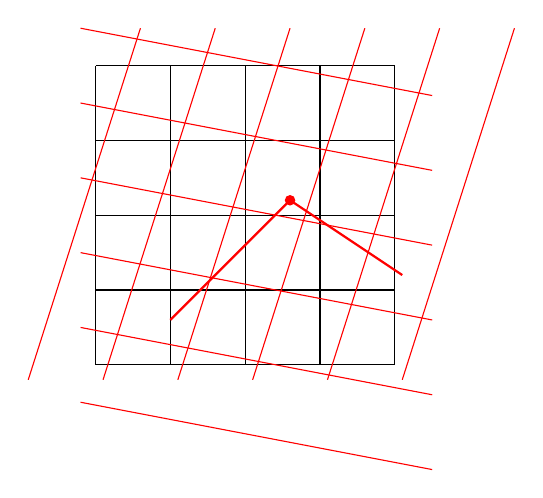
\begin{tikzpicture}[scale=0.95]
\draw[step=1, black, thin] (0,0) grid (4,4);
\foreach \k in {-1,0,1,2,3,4}
  \draw[red, thin] (\k+0.1,-0.2) -- (\k+1.6,4.5);
\foreach \k in {-1,0,1,2,3,4}
  \draw[red, thin] (-0.2,\k+0.5) -- (4.5,\k-0.4);
\fill[red] (2.6,2.2) circle (2pt);
\draw[red, thick] (1.0,0.6) -- (2.6,2.2);
\draw[red, thick] (2.6,2.2) -- (4.1,1.2);
\end{tikzpicture}
\caption{A clean schematic of the same idea: the geometry stays fixed while the coordinate families change.}
\end{figure}

A scalar is the simplest case. It has no directional content. If the \(x\)-coordinates and the \(y\)-coordinates label the same point, then the scalar has the same value in both descriptions:
\begin{equation}
\phi(y)=\phi(x).
\end{equation}
That is not yet deep tensor calculus; it is the statement that everybody agrees on the temperature at a given point, no matter how they coordinatize space.

\begin{figure}[h]
\centering

\includegraphics[width=0.7\textwidth]{lecture_03_figure_03.png}
\caption{Scalar equality and free vector. The board places scalar invariance and the geometric displacement side by side.}
\end{figure}

\begin{figure}[h]
\centering
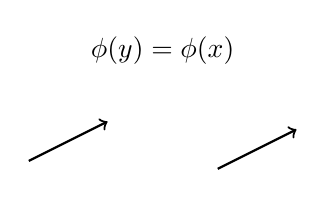
\begin{tikzpicture}[scale=1.0]
\node at (2.5,2.2) {$\phi(y)=\phi(x)$};
\draw[->, thick] (0.8,0.8) -- (1.8,1.3);
\draw[->, thick] (3.2,0.7) -- (4.2,1.2);
\end{tikzpicture}
\caption{Schematic redraw of the board's point: the scalar is unchanged, while the same free vector may be drawn at different locations without altering the geometric object.}
\end{figure}

The primordial vector in the lecture is the infinitesimal displacement. One may think of it as a little arrow, but what matters is that its components in the \(x\)-system are \(dx^{m}\), whereas its components in the \(y\)-system are \(dy^{n}\). Since \(y^{n}\) is itself an ordinary function of the \(x\)'s, we may apply the total-differential formula to \(y^{n}\) itself:
\begin{equation}
dy^{n}=\frac{\partial y^{n}}{\partial x^{m}}\,dx^{m}.
\end{equation}

\begin{definition}
A contravariant vector is a collection of components \(V^{m}\) whose components in two coordinate systems are related by
\begin{equation}
V^{n}_{(y)}=\frac{\partial y^{n}}{\partial x^{m}}\,V^{m}_{(x)}.
\end{equation}
The infinitesimal displacement \(dx^{m}\) is the model example.
\end{definition}

The lecture then builds higher-rank tensors constructively. If \(A^{m}\) and \(B^{n}\) are vectors, then the products \(A^{m}B^{n}\) form the components of a rank-two object. Each index transforms the same way the original vector index transformed, so each index brings its own Jacobian factor.

Next comes the other kind of vector. The collection \(\partial \phi/\partial x^{m}\) also has \(d\) components, but it is not a displacement. It is the gradient of a scalar. Its transformation law is read directly from the chain rule:

\begin{definition}
A covariant vector is a collection of components \(A_{m}\) whose components transform according to
\begin{equation}
A^{(y)}_{n}=\frac{\partial x^{m}}{\partial y^{n}}\,A^{(x)}_{m}.
\end{equation}
The gradient \(\partial \phi/\partial x^{m}\) is the lecture's model example.
\end{definition}

This is where the upstairs and downstairs notation becomes useful. Contravariant indices are written upstairs, covariant indices downstairs. The rule for contractions is then easy to inspect visually: one sums an upstairs index against a downstairs one. In the lecture this is still presented mainly as disciplined bookkeeping, but it is a very powerful bookkeeping device.

A rank-two tensor with two lower indices transforms by one factor of \(\partial x/\partial y\) for each index:
\begin{equation}
T^{(y)}_{mn}
=
\frac{\partial x^{r}}{\partial y^{m}}
\frac{\partial x^{s}}{\partial y^{n}}
T^{(x)}_{rs}.
\end{equation}

\begin{figure}[h]
\centering

\includegraphics[width=0.65\textwidth]{lecture_03_figure_04.png}
\caption{Rank-two tensor transformation law. The board gives the clean two-index lower-index transformation rule just before the metric tensor appears.}
\end{figure}

What matters here is the pattern. A scalar has no indices and is unchanged. A contravariant vector transforms with \(\partial y/\partial x\). A covariant vector transforms with \(\partial x/\partial y\). A tensor gets one such factor for each of its indices.

\section{The Metric Tensor}

After the break the lecture begins again from the simplest possible geometry: flat space. We are not yet discussing spacetime; we are discussing space. Susskind is also careful to distinguish flat \emph{space} from flat \emph{coordinates}. A flat space may be described in curvilinear coordinates. What makes it flat is not the visual straightness of the coordinates, but the existence of some coordinate system in which the metric takes the Cartesian form.

Take an infinitesimal displacement \(dx\) in Cartesian coordinates. Its squared length is \(ds^{2}\). In ordinary flat space Pythagoras gives
\begin{equation}
ds^{2}=(dx^{1})^{2}+(dx^{2})^{2}+\cdots.
\end{equation}
To restore the upstairs-downstairs contraction pattern, Susskind introduces the Kronecker delta:
\[
\delta_{mn}=1 \quad \text{if } m=n,
\qquad
\delta_{mn}=0 \quad \text{if } m\neq n.
\]
Then the line element may be written compactly as
\begin{equation}
ds^{2}=\delta_{mn}\,dx^{m}dx^{n}.
\end{equation}
In Cartesian coordinates the metric tensor is therefore just the Kronecker delta.

\begin{figure}[h]
\centering

\includegraphics[width=0.62\textwidth]{lecture_03_figure_05.png}
\caption{Metric tensor in Cartesian coordinates. The circled \(\delta_{mn}\) marks the point at which the Kronecker delta is explicitly identified as the Cartesian metric tensor.}
\end{figure}

Now change coordinates from \(x\) to \(y\). The first step, visible on the board, is
\begin{equation}
dx^{m}=\frac{\partial x^{m}}{\partial y^{r}}\,dy^{r}.
\end{equation}

\begin{figure}[h]
\centering

\includegraphics[width=0.72\textwidth]{lecture_03_figure_06.png}
\caption{Metric tensor under coordinate change. The board identifies the coefficient of \(dy^{r}dy^{s}\) as the new metric components.}
\end{figure}

The rest is simply substitution.

\begin{proposition}
If
\[
ds^{2}=g^{(x)}_{mn}\,dx^{m}dx^{n},
\]
then under a coordinate transformation \(x=x(y)\), the metric components in the \(y\)-system are
\begin{equation}
g^{(y)}_{rs}
=
g^{(x)}_{mn}
\frac{\partial x^{m}}{\partial y^{r}}
\frac{\partial x^{n}}{\partial y^{s}}.
\end{equation}
In particular, the metric is a covariant tensor of rank \(2\).
\end{proposition}

\begin{proof}
We substitute the differential transformation law into the line element:
\begin{align}
ds^{2}
&=
g^{(x)}_{mn}\,dx^{m}dx^{n} \\
&=
g^{(x)}_{mn}
\left(\frac{\partial x^{m}}{\partial y^{r}}\,dy^{r}\right)
\left(\frac{\partial x^{n}}{\partial y^{s}}\,dy^{s}\right) \\
&=
\left(
g^{(x)}_{mn}
\frac{\partial x^{m}}{\partial y^{r}}
\frac{\partial x^{n}}{\partial y^{s}}
\right)dy^{r}dy^{s}.
\end{align}
The parenthesized coefficient is exactly the object Susskind circles on the board. By definition we call it \(g^{(y)}_{rs}\). Since each lower index brings a factor of \(\partial x/\partial y\), the metric transforms as a covariant rank-two tensor.
\end{proof}

This is the first major geometric payoff of the tensor machinery. The metric is the object that tells us the distance between neighboring points,
\begin{equation}
ds^{2}=g_{mn}(x)\,dx^{m}dx^{n}.
\end{equation}
Once we know the metric, we know the local geometry.

\section{Flatness, Curvature, and Worked Examples}

The lecture now turns from algebra back to geometry. Suppose someone hands us a collection of functions \(g_{mn}(x)\). When does that metric describe flat space, and when does it describe curved space? Susskind's answer is operational and coordinate-based.

\begin{definition}
A space is flat if there exists some coordinate system in which the metric takes the Cartesian form
\[
g_{mn}=\delta_{mn}.
\]
If no coordinate transformation can bring the metric to that form, the space is curved. Curvature is thus an obstruction to flattening the metric globally.
\end{definition}

This notion of obstruction echoes the earlier physics exactly. Just as tidal forces obstruct the global removal of gravity, curvature obstructs the global straightening of the metric. One can often do better locally than globally: a curved space can be flattened in an infinitesimal neighborhood of a point, and sometimes over an extended patch, without being globally flat. The cone is the lecture's sharp example. Any patch away from the tip can be opened out flat, but the tip itself obstructs a single global flattening.

\paragraph{Worked example: polar coordinates in the plane.} The next example is deliberately concrete. Start with flat two-dimensional space and replace Cartesian coordinates by polar coordinates:
\begin{equation}
x=r\cos\theta,
\qquad
y=r\sin\theta.
\end{equation}
Differentiate:
\begin{align}
dx &= \cos\theta\,dr-r\sin\theta\,d\theta, \\
dy &= \sin\theta\,dr+r\cos\theta\,d\theta.
\end{align}
Now substitute into the flat line element \(ds^{2}=dx^{2}+dy^{2}\):
\begin{align}
ds^{2}
&=
\left(\cos\theta\,dr-r\sin\theta\,d\theta\right)^{2}
+
\left(\sin\theta\,dr+r\cos\theta\,d\theta\right)^{2} \\
&=
\left(\cos^{2}\theta+\sin^{2}\theta\right)dr^{2}
+
r^{2}\left(\sin^{2}\theta+\cos^{2}\theta\right)d\theta^{2}
+
0\cdot dr\,d\theta \\
&=
dr^{2}+r^{2}d\theta^{2}.
\end{align}
So the metric components are
\begin{equation}
g_{rr}=1,
\qquad
g_{r\theta}=0,
\qquad
g_{\theta\theta}=r^{2}.
\end{equation}

The important point is not merely the formula but the interpretation. The metric is no longer a constant array of zeros and ones, even though the underlying space is still flat. The complexity can come from the coordinate system, not from the intrinsic geometry.

\subsection{Question \& Answer}

\paragraph{Question.} What does the vanishing off-diagonal term actually tell us?

\paragraph{Answer.} In this example it tells us something about the coordinates, not something decisive about the space by itself. The absence of a cross term means that the lines of constant \(r\) and the lines of constant \(\theta\) are perpendicular to one another. Here those are circles and radial rays, respectively. If we had chosen more complicated curvilinear coordinates whose coordinate lines were not orthogonal, then a mixed term \(g_{r\theta}\,dr\,d\theta\) would generally appear. So \(g_{r\theta}=0\) reflects an orthogonality property of the chosen coordinates; it is not, by itself, a proof of flatness.

At the very end of the lecture Susskind turns to the sphere. The transcript becomes unreliable in the surrounding verbal explanation, so the safest course is to record only the mathematical statement that is clearly intended. For a unit sphere, in the late notation of the lecture, the metric is
\begin{equation}
ds^{2}=d\phi^{2}+\sin^{2}\phi\,d\theta^{2}.
\end{equation}
Here the symbol \(\phi\) is no longer the earlier scalar field; it is now an angular coordinate on the sphere. The point of the example is not the derivation on the board, which is only partially recoverable from the transcript, but the geometric fact: unlike the plane in polar coordinates, the sphere cannot be globally straightened so that the metric becomes the Kronecker delta. That impossibility is the curvature.

\begin{remark}
The sphere discussion in the transcript is badly garbled in its final minutes. The standard unit-sphere metric written above is consistent with the lecture's intent, but the surrounding derivation should be treated cautiously.
\end{remark}

\section{Summary}

The lecture begins with a physical puzzle about light in an elevator and ends with the metric tensor. The path is not accidental. A vertical light ray reveals gravitational red shift and blue shift; free fall reveals the local cancellation demanded by the equivalence principle; tidal forces reveal the obstruction that survives any local coordinate trick. That obstruction then reappears in geometry as curvature.

The mathematical development is deliberately cumulative. We start with the total differential and the chain rule, package coordinate change into transformation laws, distinguish scalars from vectors and covectors, and then identify the metric as a covariant tensor of rank \(2\). Once the metric is in hand, flatness means that some coordinate system restores the Kronecker-delta form. When no such global restoration exists, the obstruction has become geometry itself.